\documentclass[main.tex]{subfiles}
\begin{document}


\section{Uniforme continuiteit}
\label{sec:unif-cont}

\begin{tvb}
  Zij een continue functie $f: \interval[open left]{0}{1} \rightarrow \mathbb{R}$, dan bestaat er niet steeds een continue uitbreiding $g$ van $f$ naar $\interval{0}{1}$.

  \begin{proof}
    Beschouw de functie $f$ als volgt, dan bestaat er geen continue uitbreiding $g$ van $f$ naar $\interval{0}{1}$.
    \[ f:\ \interval[open left]{0}{1} \rightarrow \mathbb{R}:\ x \mapsto \frac{1}{x} \]
    \begin{figure}[H]
      \centering
      \begin{tikzpicture}[scale=0.5]
        \begin{axis}[ymax=10, ymin=0, xmax=1.125, xmin=0]
          \addplot[domain=0:1] {1/x};
          \addplot[soldot] coordinates{(1,1)};
        \end{axis}
      \end{tikzpicture}
    \end{figure}
    Zij immers $g$ een continue uitbreiding van $f$ met $g(0)=c \in \mathbb{R}$.
    Kies nu $\epsilon$, dan geldt voor alle $\delta\in \mathbb{R}_{0}^{+}$ dat er een $x\in \interval[open left]{0}{1}$ bestaat die verder dan $\epsilon$ van $c$ ligt.
  \end{proof}
\end{tvb}

\begin{st}
  Zij een continue functie $f: \interval[open left]{0}{1} \rightarrow \mathbb{R}$, en $g$ een continue uitbreiding van $f$ naar $\interval{0}{1}$, dan is die uitbreiding uniek.
  
  \begin{proof}
    Opdat $g$ continu zou in $\interval{0}{1}$ moet voor elke rij $(x_{n})_{n}$ die naar nul convergeert $(f(x_{n}))_{n}$ naar $g(0)$ convergeren.\needed
    Er is dus maar \'e\'en mogelijkheid voor $g(0)$.
    \extra{dit kan beter!}
  \end{proof}
\end{st}

\begin{st}
  Zij een continue begrensde functie $f: \interval[open left]{0}{1} \rightarrow \mathbb{R}$, dan bestaat er een continue uitbreiding $g$ van $f$ naar $\interval{0}{1}$
\extra{bewijs}
\end{st}

\begin{st}
  \label{st:continue-functie-over-gesloten-deel-behoudt-cauchy}
  Zij $f:\ A \subseteq \mathbb{R} \rightarrow \mathbb{R}$ een continue functie met $A$ gesloten en $(x_{n})_{n}$ een Cauchyrij in $\mathbb{R}$, dan is $(f(x_{n}))_{n}$ ook een Cauchyrij.

  \begin{proof}
    $(x_{n})_{n}$ is een Cauchyrij en daarom convergent.\prref{pr:cauchyrij-in-R-convergeert}
    Noem $x$ de limiet van $(x_{n})_{n}$.\prref{pr:cauchyrij-in-R-convergeert}
    Omdat $A$ gesloten is, zal $x$ tot $A$ behoren.\prref{pr:gesloten-asa-elke-convergente-rij-in-A-limiet-in-A}
    Omdat $f$ continu is, zal $f(x)$ de limiet zijn van $(f(x_{n}))_{n}$.\prref{pr:continu-asa-behoudt-convergentie}
    $(f(x_{n}))_{n}$ convergeert dus ook en is bijgevolg een Cauchyrij.\prref{pr:convergent-dan-cauchy}
  \end{proof}
\end{st}

\begin{tvb}
  Bovenstaande stelling geldt niet voor een niet-gesloten interval $A$.

  \begin{proof}
    Zij $f$ de volgende continu\"e functie:
    \[ f: \interval[open left]{0}{1} \subseteq \mathbb{R} \rightarrow \mathbb{R}:\ x \mapsto \frac{1}{x} \]
    Zij $(x_{n})_{n}$ bovendien de volgende Cauchyrij:
    \[ x_{n} = \frac{1}{n} \]
    $(f(x_{n}))_{n}$ is dan geen cauchyrij want $(f(x_{n}))_{n} = (n)_{n}$ is niet convergent.\prref{pr:cauchyrij-in-R-convergeert}
  \end{proof}
\end{tvb}

\begin{de}
  We noemen een functie $f: A \subseteq \mathbb{R} \rightarrow \mathbb{R}$ \term{uniform continu} of \term{gelijkmatig continu} op $A$ als het volgende geldt:
  \[ \forall \epsilon \in \mathbb{R}_{0}^{+}:\ \exists \delta \in \mathbb{R}_{0}^{+}:\ \forall x,y \in A:\ |x-y| < \delta \Rightarrow |f(x)-f(y)| < \epsilon \]
\end{de}



\begin{vb}
  De functie $f$ is uniform continu:
  \[ f:\ \mathbb{R} \rightarrow \mathbb{R}:\ x \mapsto \frac{x}{1+x^{2}} \]
  \extra{bewijs p 21}
\end{vb}

\begin{vb}
  De functie $f$ is uniform continu:
  \[ f:\ \mathbb{R}^{+} \rightarrow \mathbb{R}:\ x \mapsto \sqrt{x} \]

  \begin{proof}
    Merk allereerst de volgende ongelijkheid op:
    \[ |\sqrt{x} - \sqrt{y}| \le \sqrt{|x-y|} \]
    Kies een willekeurige $\epsilon$ en definieer $\delta = \epsilon^{2}$.
    Kies nu twee willekeurige elementen $x$ en $y$ uit $\mathbb{R}^{+}$ zodat $|x-y|< \delta$ geldt.
    \[ |f(x) - f(y)| \le  \sqrt{|x-y|} < \sqrt{\delta} = \sqrt{\epsilon^{2}} = \epsilon \]
    $f$ is dus uniform continu over $\mathbb{R}^{+}$.
  \end{proof}
\end{vb}

\begin{tvb}
  De functie $f$ is \textbf{niet} uniform continu:
  \[ f:\ \mathbb{R}_{0}^{+} \rightarrow \mathbb{R}:\ x \mapsto \frac{1}{x} \]

  \begin{proof}
    Kies $\epsilon = 1$ en kies een willekeurige $\delta \in \mathbb{R}_{0}^{+}$.
    Stel bovendien $y = x + \frac{\delta}{2}$, dan is $|x-y|$ altijd kleiner dan $\delta$.
    Merk bovendien de volgende gelijkheid op:
    \[ |f(x)-f(y)| = \left| \frac{1}{x} - \frac{1}{y} \right| \le \left| \frac{1}{x} - \frac{1}{x + \frac{\delta}{2}} \right| = \left| \frac{x+\frac{\delta}{2}-x}{x(x+\frac{\delta}{2})}\right| = \left| \frac{\delta}{x(2x+\delta)} \right| = \frac{\delta}{x(2x+\delta)} \]
    Kies bijvoorbeeld $x = \frac{\delta}{4}\left(\sqrt{1+\frac{\delta}{4}}-1\right)$ (de oplossing van $\frac{1}{2}(2x^{2}+\delta x) = \delta$).
    $x$ is dan positief en $|f(x)-f(y)| = 2 > \epsilon$.
    $f$ is dus niet uniform continu op $\mathbb{R}_{0}^{+}$.
  \end{proof}
\end{tvb}

\begin{vb}
  De functie $f$ is uniforum continu:
  \[ f:\ \interval[open]{1}{+\infty} \rightarrow \mathbb{R}:\ x \mapsto \frac{1}{x} \]
    \begin{figure}[H]
      \centering
      \begin{tikzpicture}[scale=0.5]
        \begin{axis}[xmin=0.9, xmax=5, ymin=0, ymax=2]
          \addplot[domain=1:10,smooth] {1/x};
          \addplot[soldot] coordinates{(1,1)};
        \end{axis}
      \end{tikzpicture}
    \end{figure}

    \begin{proof}
      Kies een willekeurige $\epsilon \in \mathbb{R}_{0}^{+}$ en merk het volgende op:
      \[ \forall x,y \in \interval[open]{1}{+\infty}:\ |f(x)-f(y)| = \left|\frac{1}{x}- \frac{1}{y}\right| = \frac{|x-y|}{|x||y|} \le |x-y| \]
      Kies nu $\delta = \epsilon$.
      \[ |f(x)-f(y)| \le |x-y| < \delta = \epsilon \]
      $f$ is dus uniform continu op $\interval[open]{1}{+\infty}$.
    \end{proof}
\end{vb}


\begin{tvb}
  De functie $f$ is \textbf{niet} uniform continu op $\mathbb{R}$:
  \[ f:\ \mathbb{R} \rightarrow \mathbb{R}:\ x \mapsto x^{2}\]
  \extra{bewijs p 22}
\end{tvb}

\begin{vb}
  De functie $f$ is uniforum continu op:
  \[ f:\ \interval[open]{-1}{1} \rightarrow \mathbb{R}:\ x \mapsto x^{2}\]
    \begin{figure}[H]
      \centering
      \begin{tikzpicture}[scale=0.5]
        \begin{axis}[xmin=-1.1, xmax=1.1, ymin=0, ymax=2]
          \addplot[domain=-1:1,smooth] {x^2};
          \addplot[holdot] coordinates{(-1,1)(1,1)};
        \end{axis}
      \end{tikzpicture}
    \end{figure}

  \begin{proof}
      Kies een willekeurige $\epsilon \in \mathbb{R}_{0}^{+}$ en merk het volgende op:
      \[ \forall x,y \in \interval[open]{-1}{1}:\ |f(x)-f(y)| = \left|x^{2}- y^{2}\right| = |x-y||x+y| < 2|x-y| \]
      Kies nu $\delta = \frac{1}{2}\epsilon$
      \[ |f(x)-f(y)| \le 2|x-y| < 2\delta = \frac{1}{2}2\epsilon = \epsilon\]
      $f$ is dus uniforum continu op $\interval[open]{-1}{1}$
  \end{proof}
\end{vb}

\begin{tvb}
  De functie $f$ is \textbf{niet} uniforum continu op $\mathbb{R}$:
  \[ f:\ \mathbb{R} \rightarrow \mathbb{R}:\ x \mapsto x^{3} \]
    \begin{figure}[H]
      \centering
      \begin{tikzpicture}[scale=0.5]
        \begin{axis}[xmin=-2, xmax=2, ymin=-3, ymax=3]
          \addplot[domain=-3:3,smooth] {x^3};
        \end{axis}
      \end{tikzpicture}
    \end{figure}
    \begin{proof}
      Kies $\epsilon = 1$ en een willekeurige $\delta \in \mathbb{R}_{0}^{+}$.
      Kies $x, y \in \mathbb{R}$ met $y=x + \frac{\delta}{2}$.
      \[
      |f(x)-f(y)|
      = \left| x^{3}-y^{3}\right|
      \]
\extra{bewijs}
    \end{proof}
\end{tvb}

\begin{vb}
  De functie $f$ is uniforum continu:
  \[ f:\ \interval[open]{-1}{1} \rightarrow \mathbb{R}:\ x \mapsto x^{3} \]
    \begin{figure}[H]
      \centering
      \begin{tikzpicture}[scale=0.5]
        \begin{axis}[xmin=-1.5, xmax=1.5, ymin=-1.5, ymax=1.5]
          \addplot[domain=-1:1,smooth] {x^3};
          \addplot[holdot] coordinates{(-1,-1)(1,1)};
        \end{axis}
      \end{tikzpicture}
    \end{figure}
\end{vb}

\begin{vb}
  De functie $f$ is uniforum continu:
  \[ f:\ \interval[open]{-1}{1} \rightarrow \mathbb{R}:\ x \mapsto \sin\left(\frac{1}{x}\right) \]
    \begin{figure}[H]
      \centering
      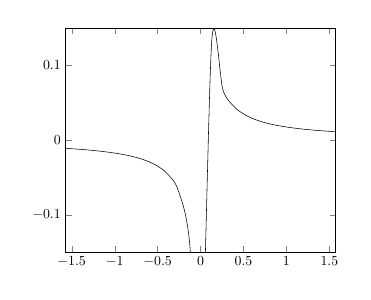
\begin{tikzpicture}[scale=0.5]
        \begin{axis}[xmin=-pi/2, xmax=pi/2, ymin=-.15, ymax=.15]
          \addplot[domain=-pi/2:pi/2,smooth] {sin(1/x)};
        \end{axis}
      \end{tikzpicture}
    \end{figure}
  \extra{bewijs (zodra de sinus gedefineerd is?)}
\end{vb}

\begin{vb}
  De functie $f$ is uniforum continu:
  \[ f:\ \interval[open]{-1}{1} \rightarrow \mathbb{R}:\ x \mapsto \frac{1}{1+x} \]
    \begin{figure}[H]
      \centering
      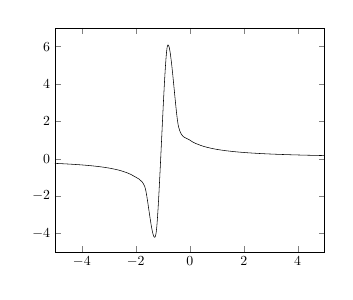
\begin{tikzpicture}[scale=0.5]
        \begin{axis}[xmin=-5, xmax=5, ymin=-5, ymax=7]
          \addplot[domain=-5:5,smooth] {1/(1+x)};
        \end{axis}
      \end{tikzpicture}
    \end{figure}
  \extra{bewijs}
\end{vb}

\begin{st}
  \label{st:uniform-continu-dan-ook-gewoon-continu}
  Als een functie $f: A \subseteq \mathbb{R} \rightarrow \mathbb{R}$ uniform continu is, is hij ook continu.
  \extra{bewijs}
\end{st}

\begin{tvb}
  Een continue functie $f: A \subseteq \mathbb{R} \rightarrow \mathbb{R}$ is niet noodzakelijk uniform continu
\extra{tegenvoorbeeld}
\end{tvb}

\begin{bpr}
  \label{pr:uniform-continue-functie-behoudt-cauchy}
  Zij $f: A \subseteq \mathbb{R} \rightarrow \mathbb{R}$ een uniform continue functie en $(x_{n})_{n}$ een Cauchyrij in $\mathbb{R}$, dan is $(f(x_{n}))_{n}$ ook een Cauchyrij.

  \begin{proof}
    Kies een willekeurige $\epsilon \in \mathbb{R}_{0}^{+}$.
    Omdat $f$ uniform continu is, bestaat er een $\delta \in \mathbb{R}_{0}^{+}$ als volgt:
    \[ \forall x,y \in A: |x-y| < \delta \Rightarrow |f(x)-f(y)| < \epsilon \]
    Omdat $(x_{n})_{n}$ een Cauchyrij is, bestaat er een $n_{0}\in \mathbb{N}$ als volgt:
    \[ \forall n,m \in \mathbb{N}: n,m \ge n_{0} \Rightarrow |x_{n}-x_{m}| < \delta \]
    Nemen we deze beweringen samen, dan bekomen we het volgende:
    \[ \forall n,m \in \mathbb{N}: n,m \ge n_{0} \Rightarrow |f(x_{n})-f(x_{m})| < \epsilon \]
    Dit betekent precies dat $(f(x_{n}))_{n}$ een Cauchyrij is.
  \end{proof}
\end{bpr}

\begin{bpr}
  Zij $f: A \subseteq \mathbb{R} \rightarrow \mathbb{R}$ een uniform continue functie.
  Als $B$ een begrensd deel is van $A$, dan is $f(B)$ ook begrensd.

  \begin{proof}
    Stel dat $f(B)$ niet begrensd zou zijn, dan kunnen we voor elke $n\in \mathbb{N}_{0}$ een $x_{n}\in B$ vinden zodat $|f(x_{n})|$ groter is dan $n$.
    We vinden zo een rij $(x_{n})_{n}$ in $B$.
    Omdat $B$ begrensd is, bestaat er een convergente deelrij $(x_{n_{k}})_{k}$.\stref{st:bolzano-rijen}
    Deze deelrij is een Cauchyrij.\prref{pr:convergent-dan-cauchy}
    De rij $(f(x_{n_{k}}))_{k}$ is dan ook een Cauchyrij.\prref{pr:uniform-continue-functie-behoudt-cauchy}
    Cauchyrijen zijn echter begrends.\prref{pr:cauchyrij-begrensd} Contradictie.
  \end{proof}
\end{bpr}

\begin{bst}
  \label{st:gesloten-en-begrensd-interval-continu-dan-uniform-continu}
  Zij $f: A \subseteq \mathbb{R} \rightarrow \mathbb{R}$ een continue functie, gedefinieerd op een gesloten en begrensd deel $A$ van $\mathbb{R}$, dan is $f$ uniform continu.

  \begin{proof}
    Stel immers dat $f$ niet uniform continu zou zijn, dan bestaat er een $\epsilon \in \mathbb{R}_{0}^{+}$ zodat we voor elke $\delta = \frac{1}{n}$ punten $x_{n}$, $y_{n}$ kunen vinden zodat het volgende geldt.
    \[ |x_{n}-y_{n}| < \frac{1}{n} \quad\wedge\quad |f(x_{n})-f(y_{n})| \ge \epsilon \]
    Omdat $(x_{n})_{n}$ een rij is in een gesloten, begrensd deel van $\mathbb{R}$ moet $(x_{n})_{n}$ begrensd zijn.
    Er bestaat daarom een deelrij $(x_{n_{k}})_{k}$ die convergeert naar een $x\in A$.\stref{st:bolzano-rijen}
    Omdat $f$ continu is, zal $(f(x_{n_{k}}))_{k}$ naar $x$ convergeren.\stref{st:continue-functie-over-gesloten-deel-behoudt-cauchy}
    Analoog vinden we een deelrij $(y_{n_{k}})_{k}$ van $(y_{n})_{n}$ die convergeert naar een $y\in A$.
    Omdat de afstand tussen $x_{n}$ en $y_{n}$ willekeurig klein wordt zal $y$ gelijk zijn aan $x$ en $f(x)$ dus ook aan $f(y)$.\stref{st:geneste-intervallen}
    We vinden dus dat de afstand tussen $f(x_{n_{k}})$ en $f(y_{n_{k}})$ willekeurig klein wordt, wat strijdig is met $|f(x_{n})-f(y_{n})| \ge \epsilon$.
    Contradictie.
\extra{dit kan beter!}
  \end{proof}
\end{bst}

\begin{st}
  Zij $f:\ \mathbb{R} \rightarrow \mathbb{R}$ een continue functie zodat het volgende geldt, dan is $f$ uniform continu op $\mathbb{R}$.
  \[ \lim_{x \rightarrow -\infty}f(x) = 0 \quad\text{ en }\quad \lim_{x \rightarrow +\infty}f(x) = 0 \]

  \begin{proof}
    Kies een willekeurige $\epsilon \in \mathbb{R}_{0}^{+}$
    Omdat de limiet van $f$ naar min oneindig $0$ is, moet er een $m_{-}\in \mathbb{R}$ bestaan zodat voor alle $x\in \mathbb{R}$ uit $x < m_{-}$ volgt dat $|f(x)| < \epsilon$ geldt.
    Analoog vinden we een $m_{+} \in \mathbb{R}$ zodat voor alle $x\in \mathbb{R}$ uit $x > m_{+}$ volgt dat $|f(x)| < \epsilon$ geldt.
    Kies nu $M = \max\{|m_{-}|,|m_{+}|\}$, dan volgt dat voor alle $x\in \mathbb{R}$ buiten $\interval{-M}{M}$, $|f(x)| < \epsilon$ geldt.\waarom
    Op het gesloten en begrensd interval $\interval{-M}{M}$ is $f$ continu en dus ook uniform continu.\stref{st:gesloten-en-begrensd-interval-continu-dan-uniform-continu}
\feed
\question{is dit voldoende? Het klinkt nogal vaag.}
  \end{proof}
\end{st}


\end{document}
